\part{Modular program design}
\frame{\partpage}

\begin{frame}[fragile]{Modular program design}
    \begin{itemize}
        \item We saw previously that \textbf{splitting your code into several files} is generally a good idea \pause
        \item Python makes it easy: any .py file can be \lstinline[language=Python]{import}ed on demand \pause
        \item C++ is a little trickier...
    \end{itemize}
\end{frame}

\begin{frame}[fragile]{Definitions and declarations}
    A function \textbf{definition} specifies its name, return type, parameters, and the code it contains:
    \begin{lstlisting}
double average(double n1, double n2)
{
    return (n1 + n2) / 2.0;
}
    \end{lstlisting}
    \pause
    A function \textbf{declaration} specifies everything \textbf{except} the code:
    \begin{lstlisting}
double average(double n1, double n2);
    \end{lstlisting}
    \pause
    A declaration tells the compiler that this function exists, but is defined \textbf{elsewhere}
\end{frame}

\begin{frame}[fragile]{Sources and headers}
    \begin{itemize}
        \item A C++ project contains two main types of file \pause
        \item \textbf{Source files} (.cpp) usually contain \textbf{definitions} \pause
        \item \textbf{Header files} (.h) usually contain \textbf{declarations} \pause
        \item For example, \texttt{myfile.cpp} may contain some function definitions,
            and \texttt{myfile.h} may contain the declarations for those functions \pause
        \item (Yep, that means you have to type the same thing twice in two different files...)
    \end{itemize}
\end{frame}

\begin{frame}[fragile]{Example}
    words.cpp
    \begin{lstlisting}
void readWords()
{
    // code omitted
}

std::string chooseRandomWord()
{
    // code omitted
}
    \end{lstlisting}
    
    words.h
    \begin{lstlisting}
#pragma once

void readWords();
std::string chooseRandomWord();
    \end{lstlisting}
\end{frame}

\begin{frame}[fragile]{Example from last week}
    \begin{itemize}
        \item \lstinline{readWords()} and \lstinline{chooseRandomWord()} are \textbf{defined} in \texttt{words.cpp} \pause
        \item \lstinline{readWords()} and \lstinline{chooseRandomWord()} are \textbf{declared} in \texttt{words.h} \pause
        \item Any file which does \lstinline{#include "words.h"} can call these functions as if they were declared in that file
    \end{itemize}
\end{frame}

\begin{frame}[fragile]{How \#include works}
    \begin{itemize}
        \item \lstinline{#include} works \textbf{exactly} as if the \lstinline{#include}d file were copied and pasted
            at the point where the \lstinline{#include} directive appears \pause
        \item All header files should start with \lstinline{#pragma once} --- otherwise,
            \lstinline{#include}ing the same file more than once will result in duplicate declaration errors \pause
        \item Putting an \lstinline{#include} directive in the wrong place (e.g.\ inside a function) will result in
            weird compile errors
    \end{itemize}
\end{frame}

\begin{frame}{The C++ build process}
	\begin{center}
		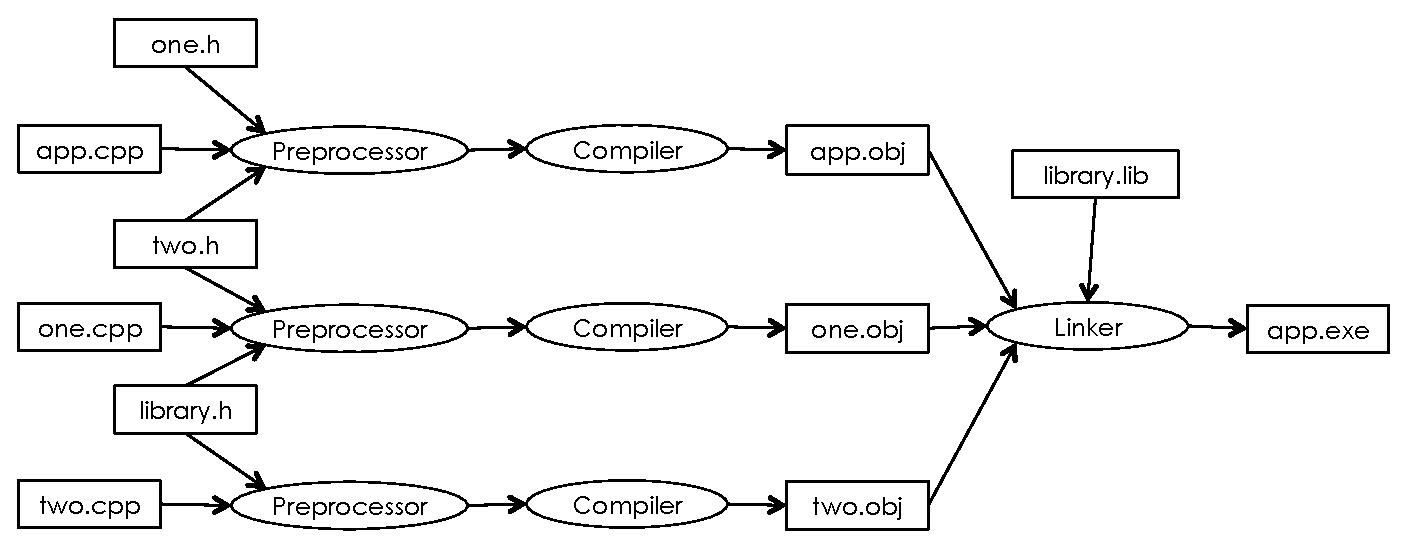
\includegraphics[width=\textwidth]{compiler_flowchart}
	\end{center}
\end{frame}

